%Optics Homework_3
\documentclass[10pt,a4paper]{article}
\usepackage[UTF8]{ctex}
\usepackage{bm}
\usepackage{amsmath}
\usepackage{extarrows}
\usepackage{amsthm}
\usepackage{amssymb}
\usepackage{graphicx}
\usepackage{multirow}
\usepackage{mathrsfs}
\title{光学作业\#3}
\author{陈稼霖 \and 45875852}
\date{2018.10.23}
\theoremstyle{remark}
\newtheorem{defi}{Definition}
\newtheorem{cdefi}{\bf 定义}
\begin{document}
\maketitle
\section*{2-29}解:
物方主面$\mathscr{H'}$和像方焦点$F'$如图(\ref{OpticsHomework_3Problem_2-29_1})。
\begin{figure}[h]
\centering
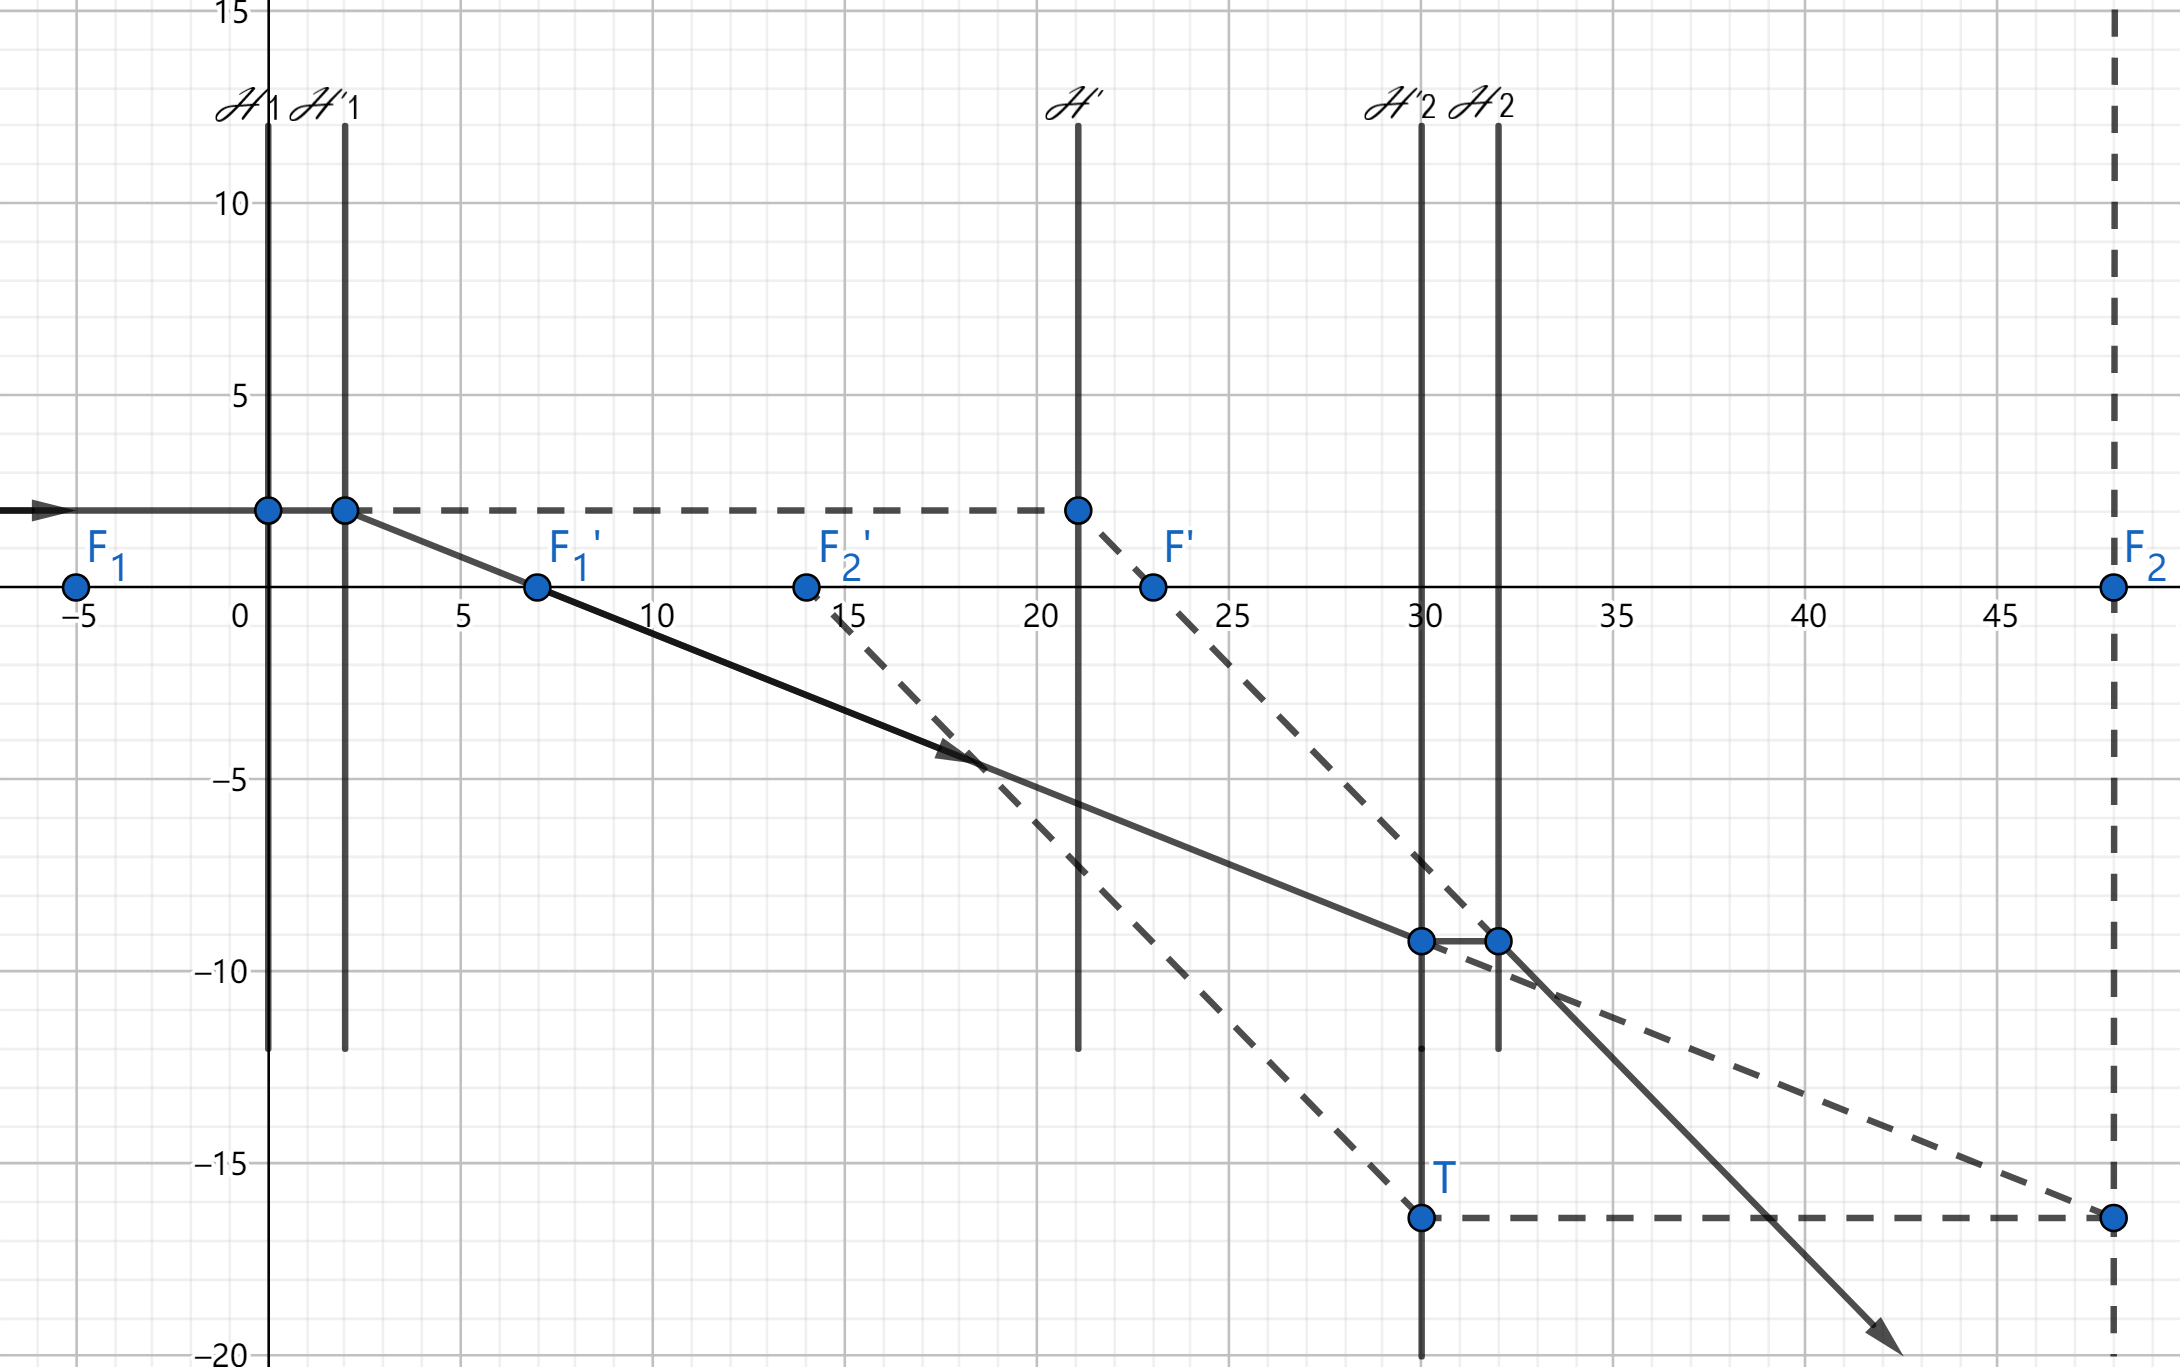
\includegraphics[scale=.25]{OpticsHomework_3Problem_2-29_1(tailored&marked).png}
\caption{题2-29图~像方主面$\mathscr{H'}$和像方焦点$F'$}\label{OpticsHomework_3Problem_2-29_1}
\end{figure}

\newpage
物方主面$\mathscr{H}$和物方焦点$F$如图(\ref{OpticsHomework_3Problem_2-29_2})。
\begin{figure}[h]
\centering
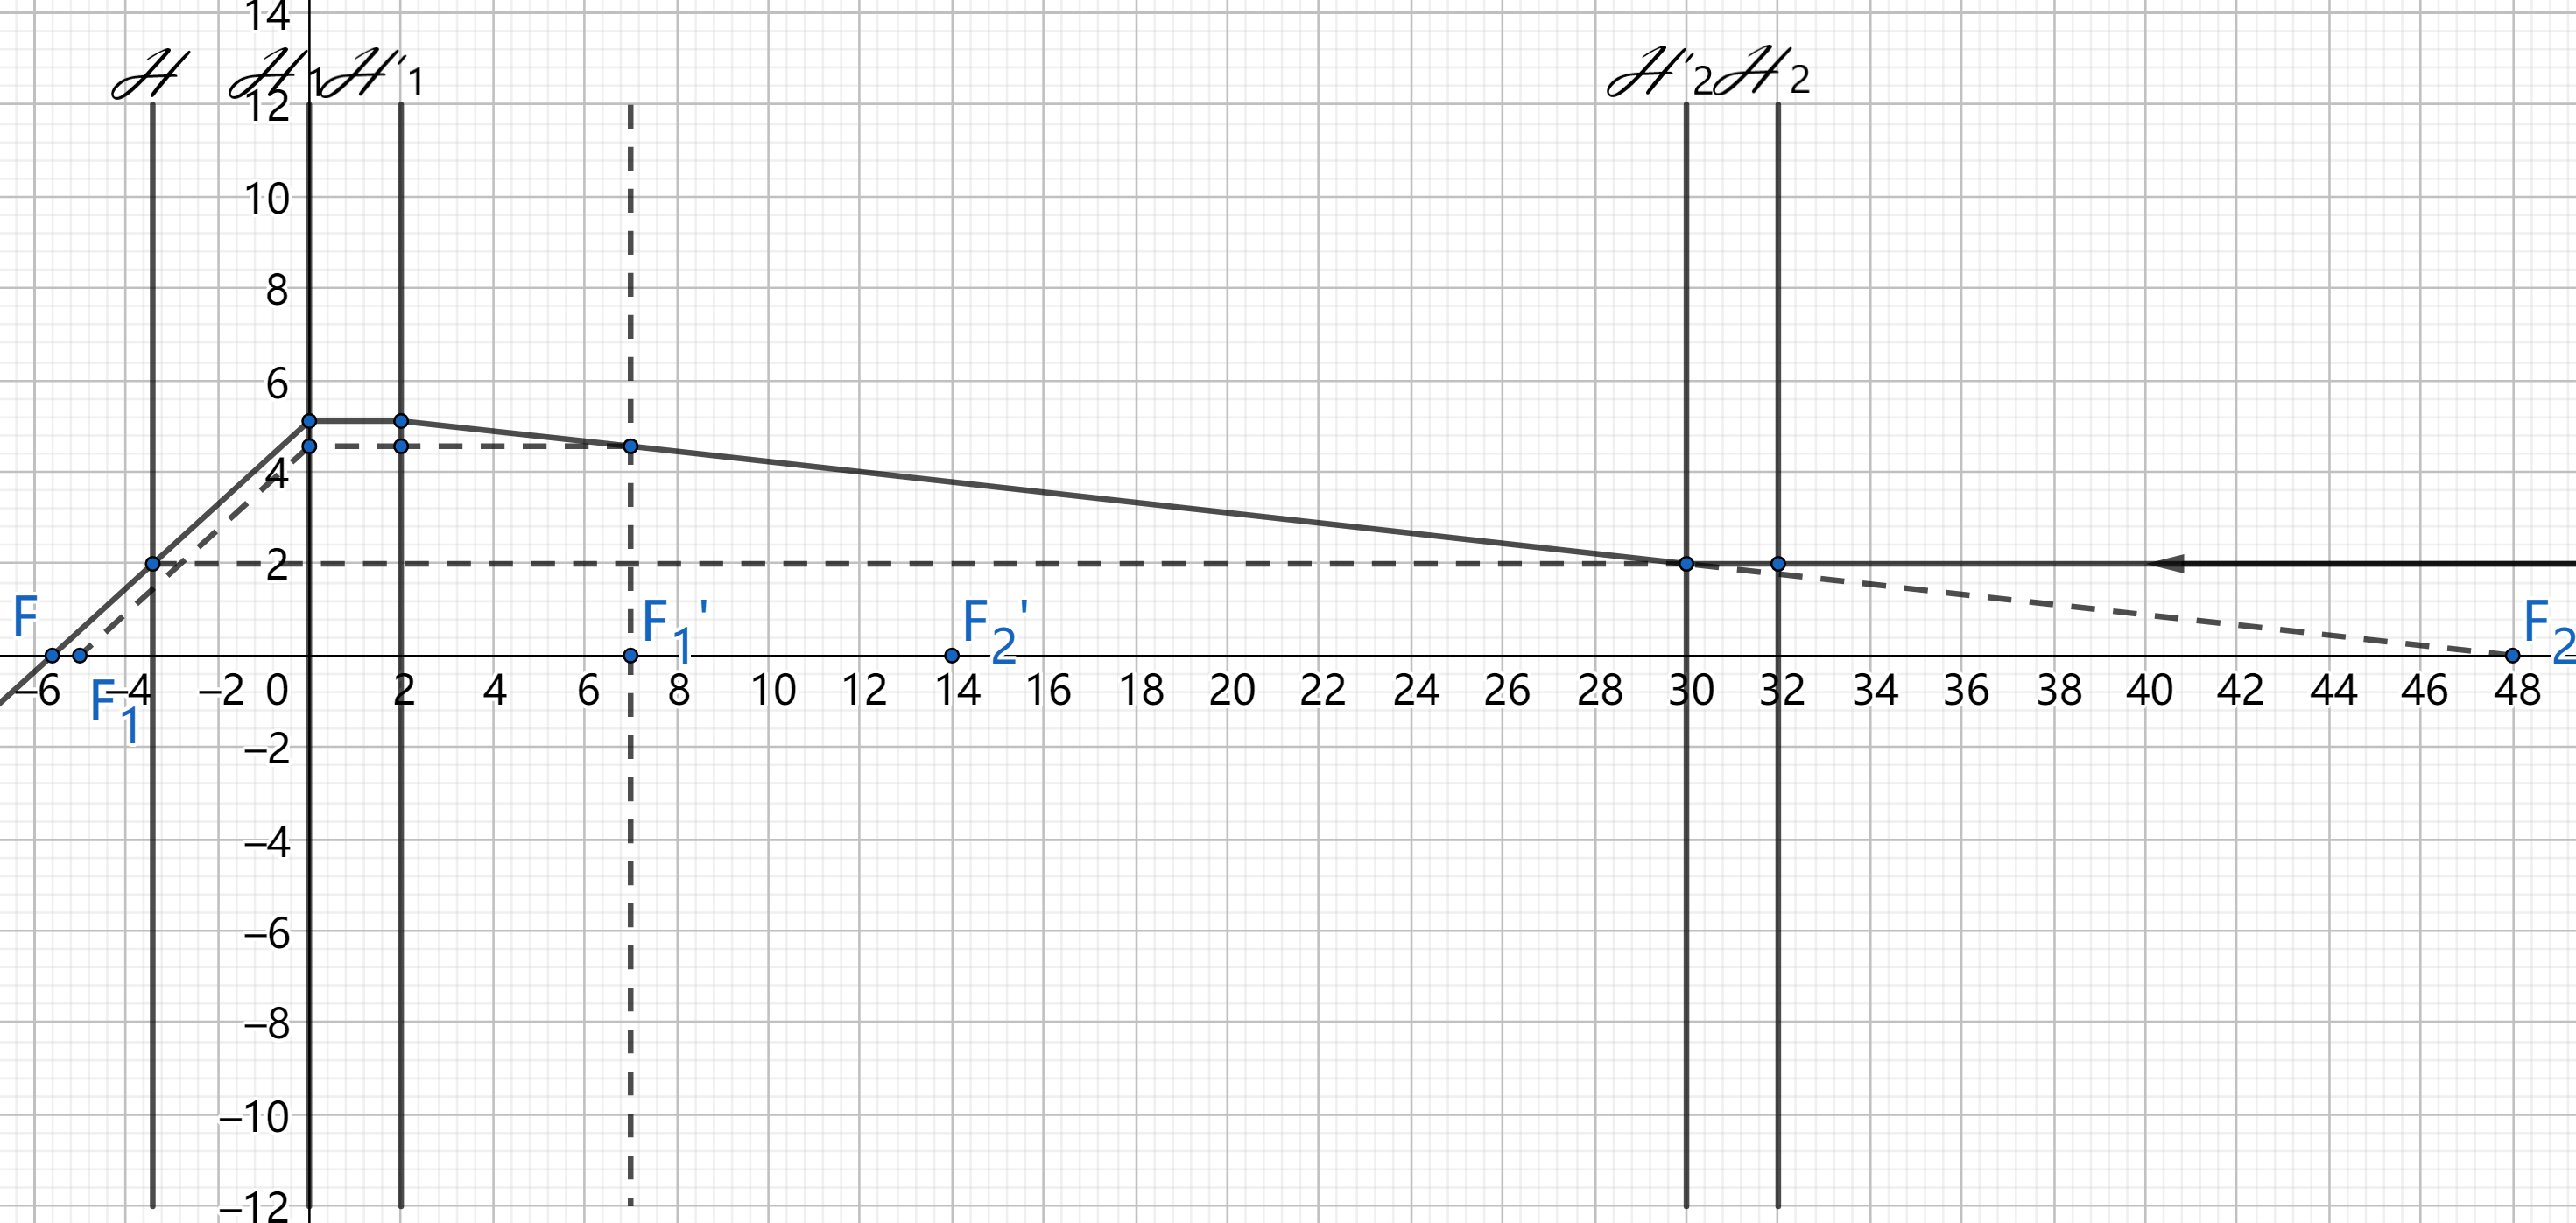
\includegraphics[scale=.2]{OpticsHomework_3Problem_2-29_2(tailored&marked).png}
\caption{题2-29图~物方主面$\mathscr{H}$和物方焦点$F$}\label{OpticsHomework_3Problem_2-29_2}
\end{figure}

\newpage
\section*{2-30}解:
如图(\ref{OpticsHomework_3Problem_2-30})。
\begin{figure}[h]
\centering
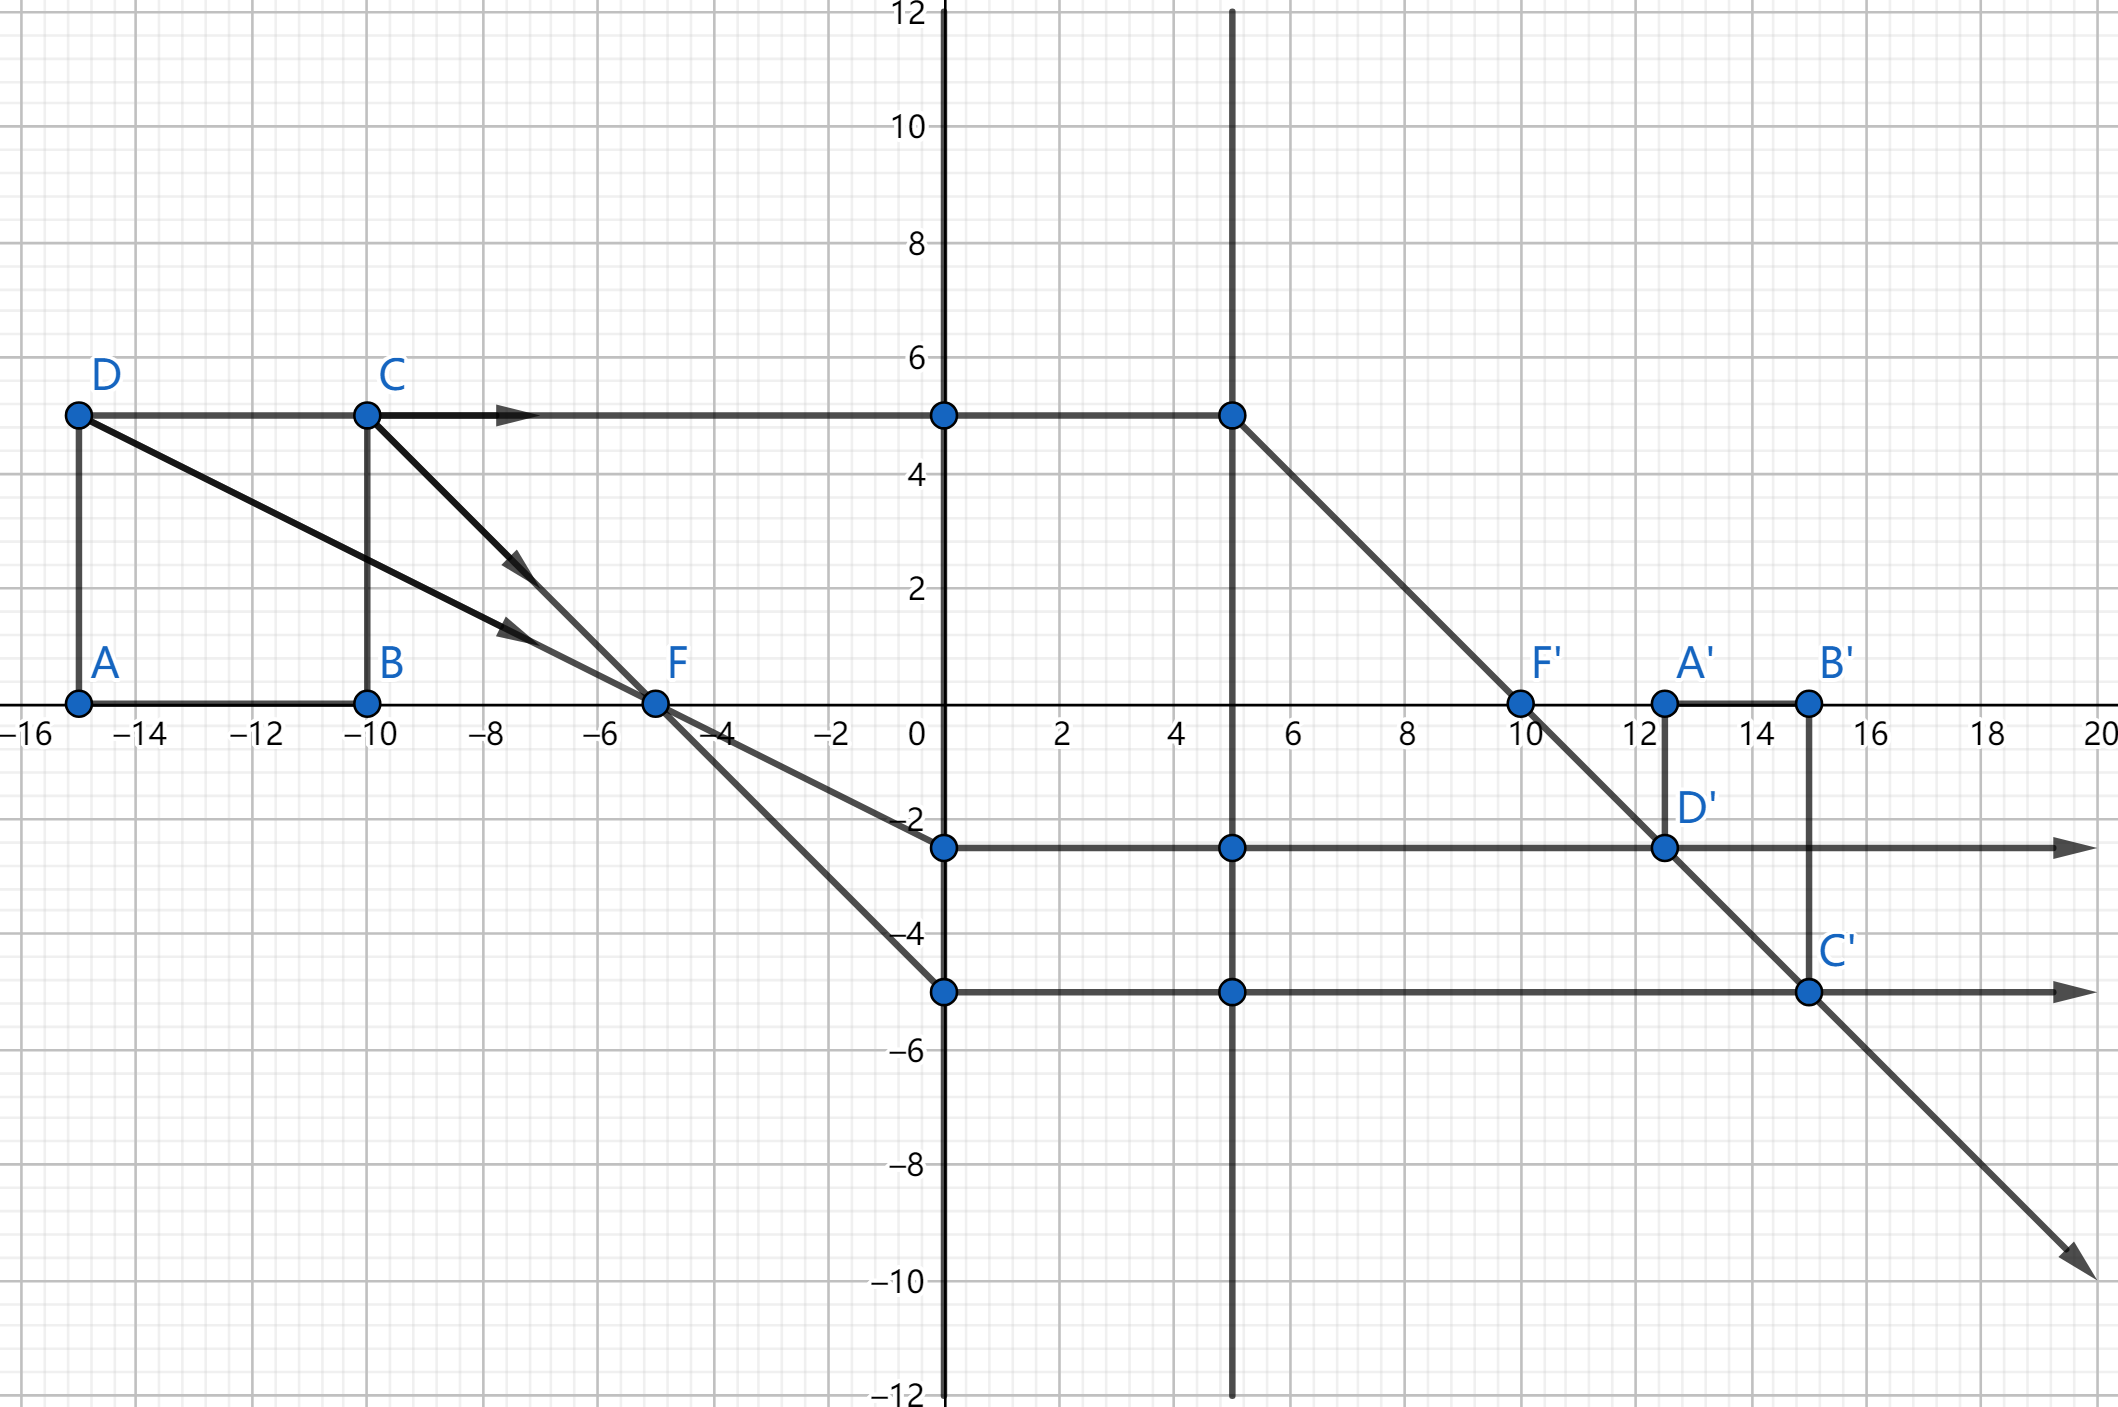
\includegraphics[scale=.25]{OpticsHomework_3Problem_2-30(tailored).png}
\caption{题2-30图}\label{OpticsHomework_3Problem_2-30}
\end{figure}

\newpage
\section*{2-32}解:
前后两折射球面的物方和像方焦距分别为
\begin{align*}
&f_1 = \frac{nr_1}{n' - n}\\
&f_1' = \frac{n'r_1}{n' - n}\\
&f_2 = \frac{n'r_2}{n - n'}\\
&f_2' = \frac{nr_2}{n - n'}
\end{align*}
两折射球面的物方和像方主点分别与其顶点重合。

\noindent 前一折射球面的像方焦点和后一物镜的物方焦点之间的距离为
\[
\Delta = d - f_1' - f_2
\]
根据理想光具组的联合公式,厚透镜的物方和像方焦距分别为
\begin{align*}
&f = -\frac{f_1f_2}{\Delta}\\
&f' = -\frac{f_1'f_2'}{\Delta}
\end{align*}
其中$f$代表厚透镜的物方焦点和前一折射球面顶点之间的距离,(设光线从左入射)若厚透镜的物方焦点在前一折射球面顶点之左,则$f > 0$,否则$f < 0$;$f'$代表厚透镜的像方焦点和后一折射球面顶点之间的距离,若厚透镜的物方焦点在后一折射球面顶点之右,则$f' > 0$,否则$f < 0$。
厚透镜的物方主点与前一折射球面物方主点(即其顶点)和像方主点和后一折射球面像方主点(即其顶点)之间的距离分别为
\begin{align*}
&X_H = f_1\frac{d}{\Delta}\\
&X_H' = f_2'\frac{d}{\Delta}
\end{align*}
其中若厚透镜的物方主点在前一折射球面的物方主点之左,则$X_H > 0$,否则$X_H < 0$;若厚透镜的像方主点在后一折射球面的像方主点之右,则$X_H > 0$,否则$X_H < 0$
\subsection*{(1)}
对于双凸透镜,代入$n = 1, n = 1.500, d = 1.00cm, r_1 = 10.0cm, r_2 = -10.0cm$,解得其
\begin{itemize}
  \item 物方焦距为$f = 10.2cm$
  \item 像方焦距为$f' = 10.2cm$
  \item 物方主点的位置为$X_H = -0.339cm$
  \item 像方主点的位置为$X_H' = -0.339cm$
\end{itemize}
物方和像方主面、物方和像方焦点$\mathscr{H},\mathscr{H}',F,F'$表示如图(\ref{OpticsHomework_3Problem2-32_1(tailored&marked)})
\subsection*{(2)}
对于双凸透镜,代入$n = 1, n = 1.500, d = 1.00cm, r_1 = 10.0cm, r_2 = 20.0cm$,解得其
\begin{itemize}
  \item 物方焦距为$f = 38.7cm$
  \item 像方焦距为$f' = 38.7cm$
  \item 物方主点的位置为$X_H = 0.645cm$
  \item 像方主点的位置为$X_H' = -1.29cm$
\end{itemize}
物方和像方主面、物方和像方焦点$\mathscr{H},\mathscr{H}',F,F'$表示如图(\ref{OpticsHomework_3Problem2-32_2(tailored&marked)})
\subsection*{(3)}
对于双凸透镜,代入$n = 1, n = 1.500, d = 1.00cm, r_1 = -15.0cm, r_2 = -20.0cm$,解得其
\begin{itemize}
  \item 物方焦距为$f = -128.6cm$
  \item 像方焦距为$f' = -128.6$
  \item 物方主点的位置为$X_H = 2.14cm$
  \item 像方主点的位置为$X_H' = -2.86$
\end{itemize}
物方和像方主面、物方和像方焦点$\mathscr{H},\mathscr{H}',F,F'$表示如图(\ref{OpticsHomework_3Problem2-32_3(enlarged&tailored&marked)})和(\ref{OpticsHomework_3Problem2-32_3(tailored&marked)})
\begin{figure}[h]
\centering
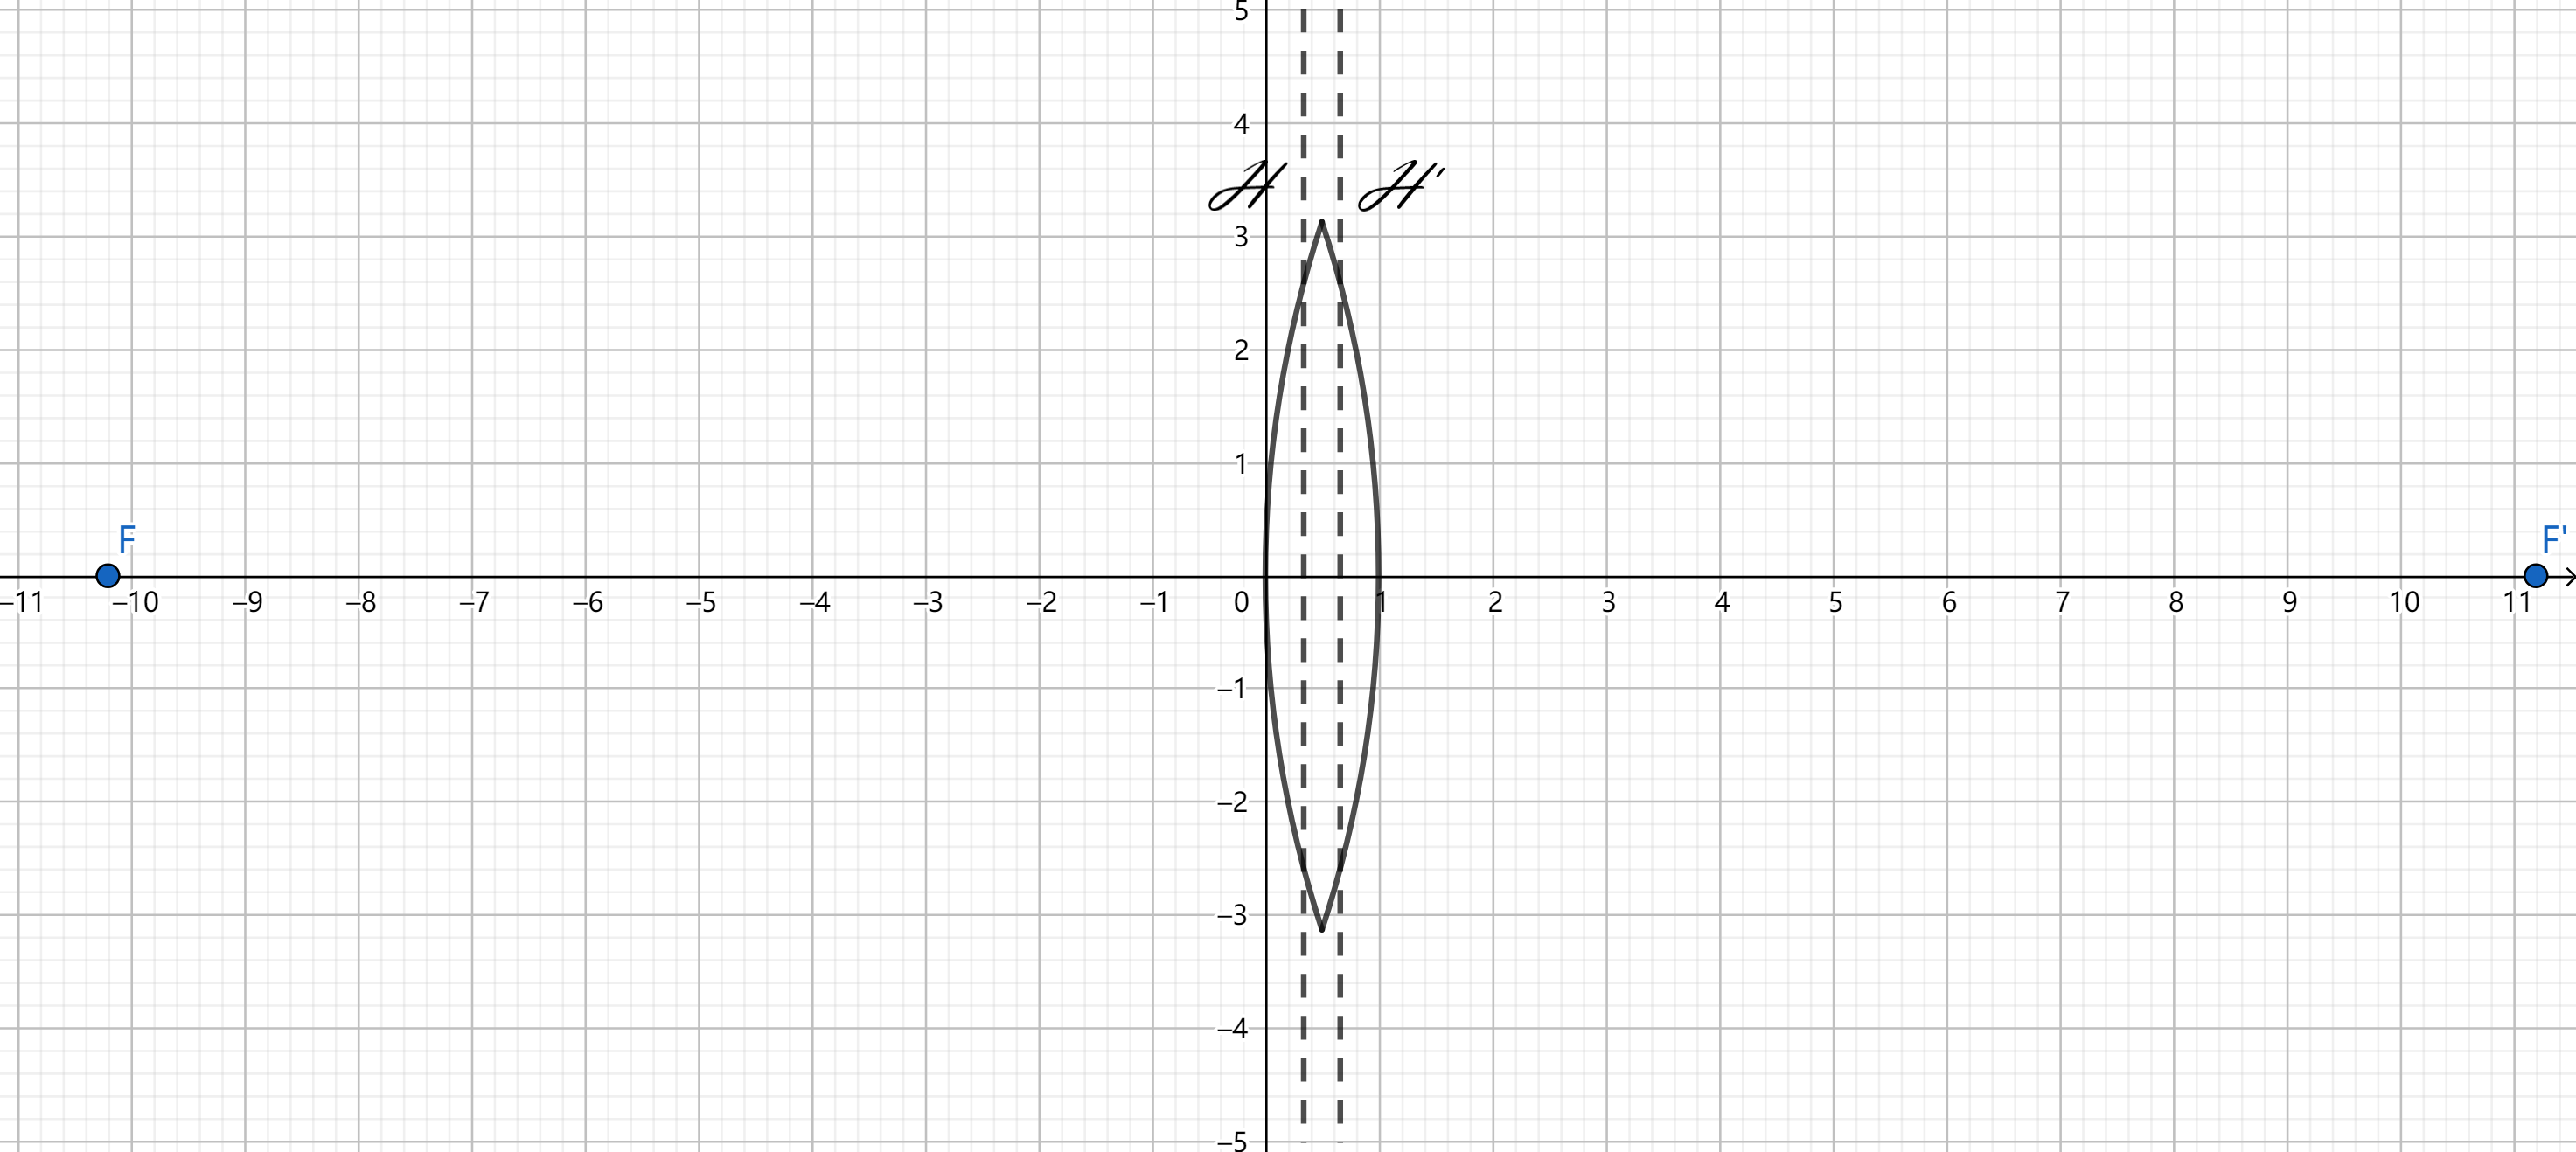
\includegraphics[scale=.2]{OpticsHomework_3Problem_2-32_1(tailored&marked).png}
\caption{题2-32图(1)物方和像方主面、物方和像方焦点$\mathscr{H},\mathscr{H}',F,F'$}\label{OpticsHomework_3Problem2-32_1(tailored&marked)}
\end{figure}
\begin{figure}[h]
\centering
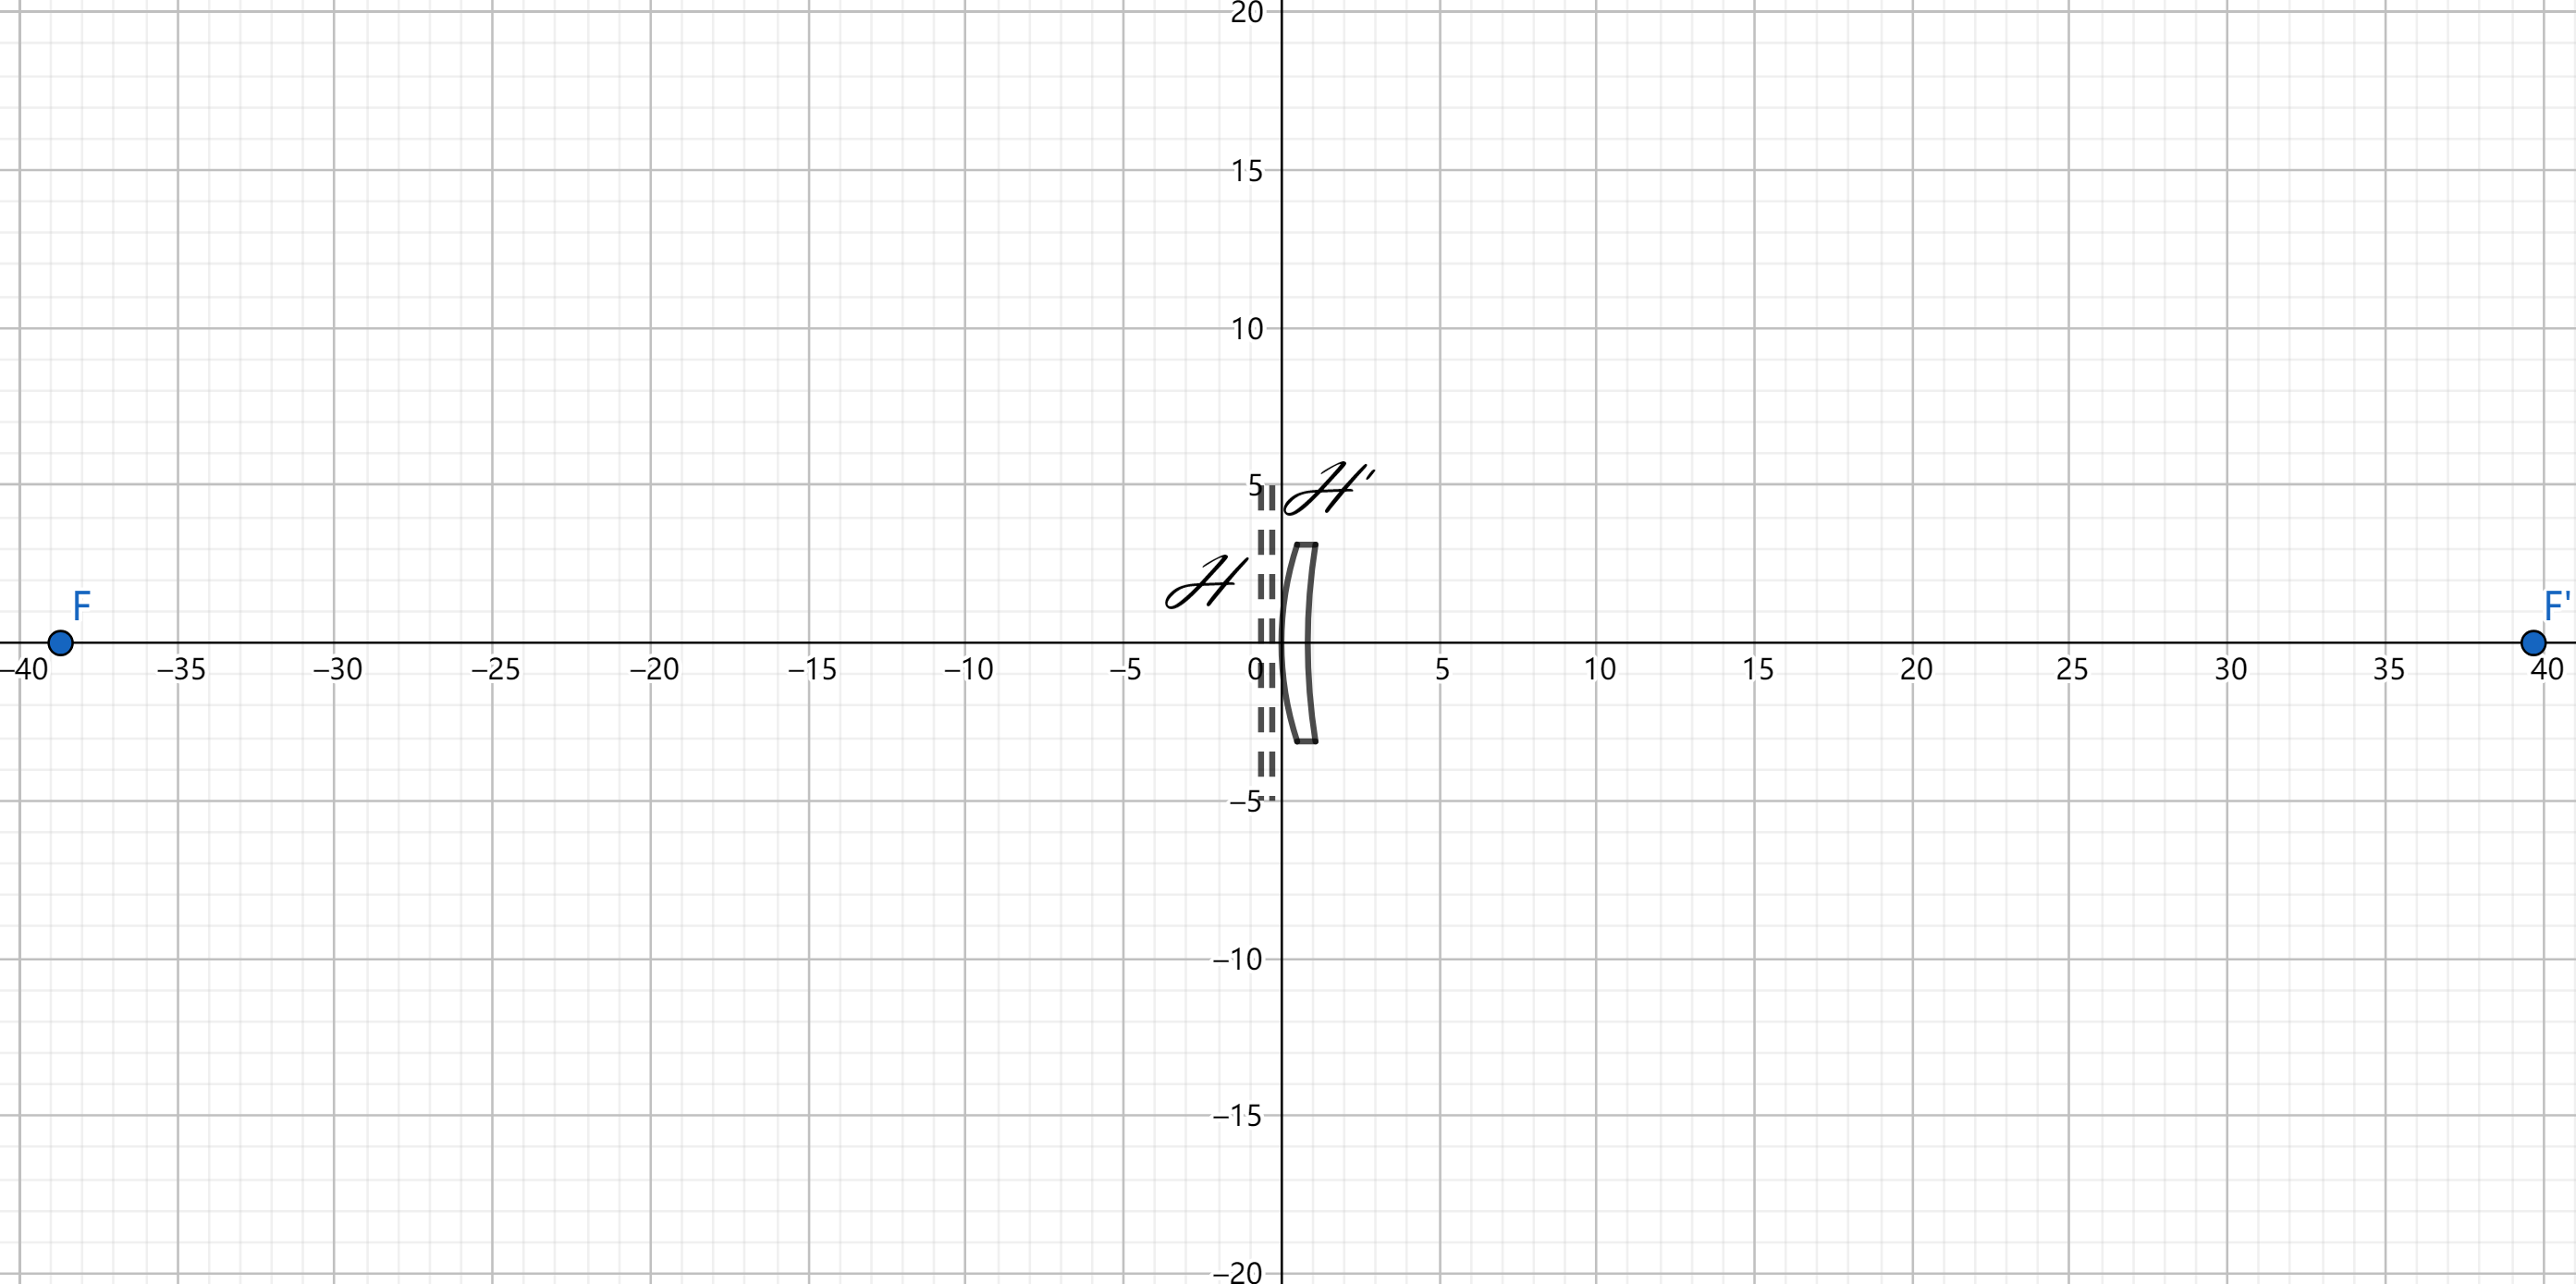
\includegraphics[scale=.2]{OpticsHomework_3Problem_2-32_2(tailored&marked).png}
\caption{题2-32图(2)物方和像方主面、物方和像方焦点$\mathscr{H},\mathscr{H}',F,F'$}\label{OpticsHomework_3Problem2-32_2(tailored&marked)}
\end{figure}
\begin{figure}[h]
\centering
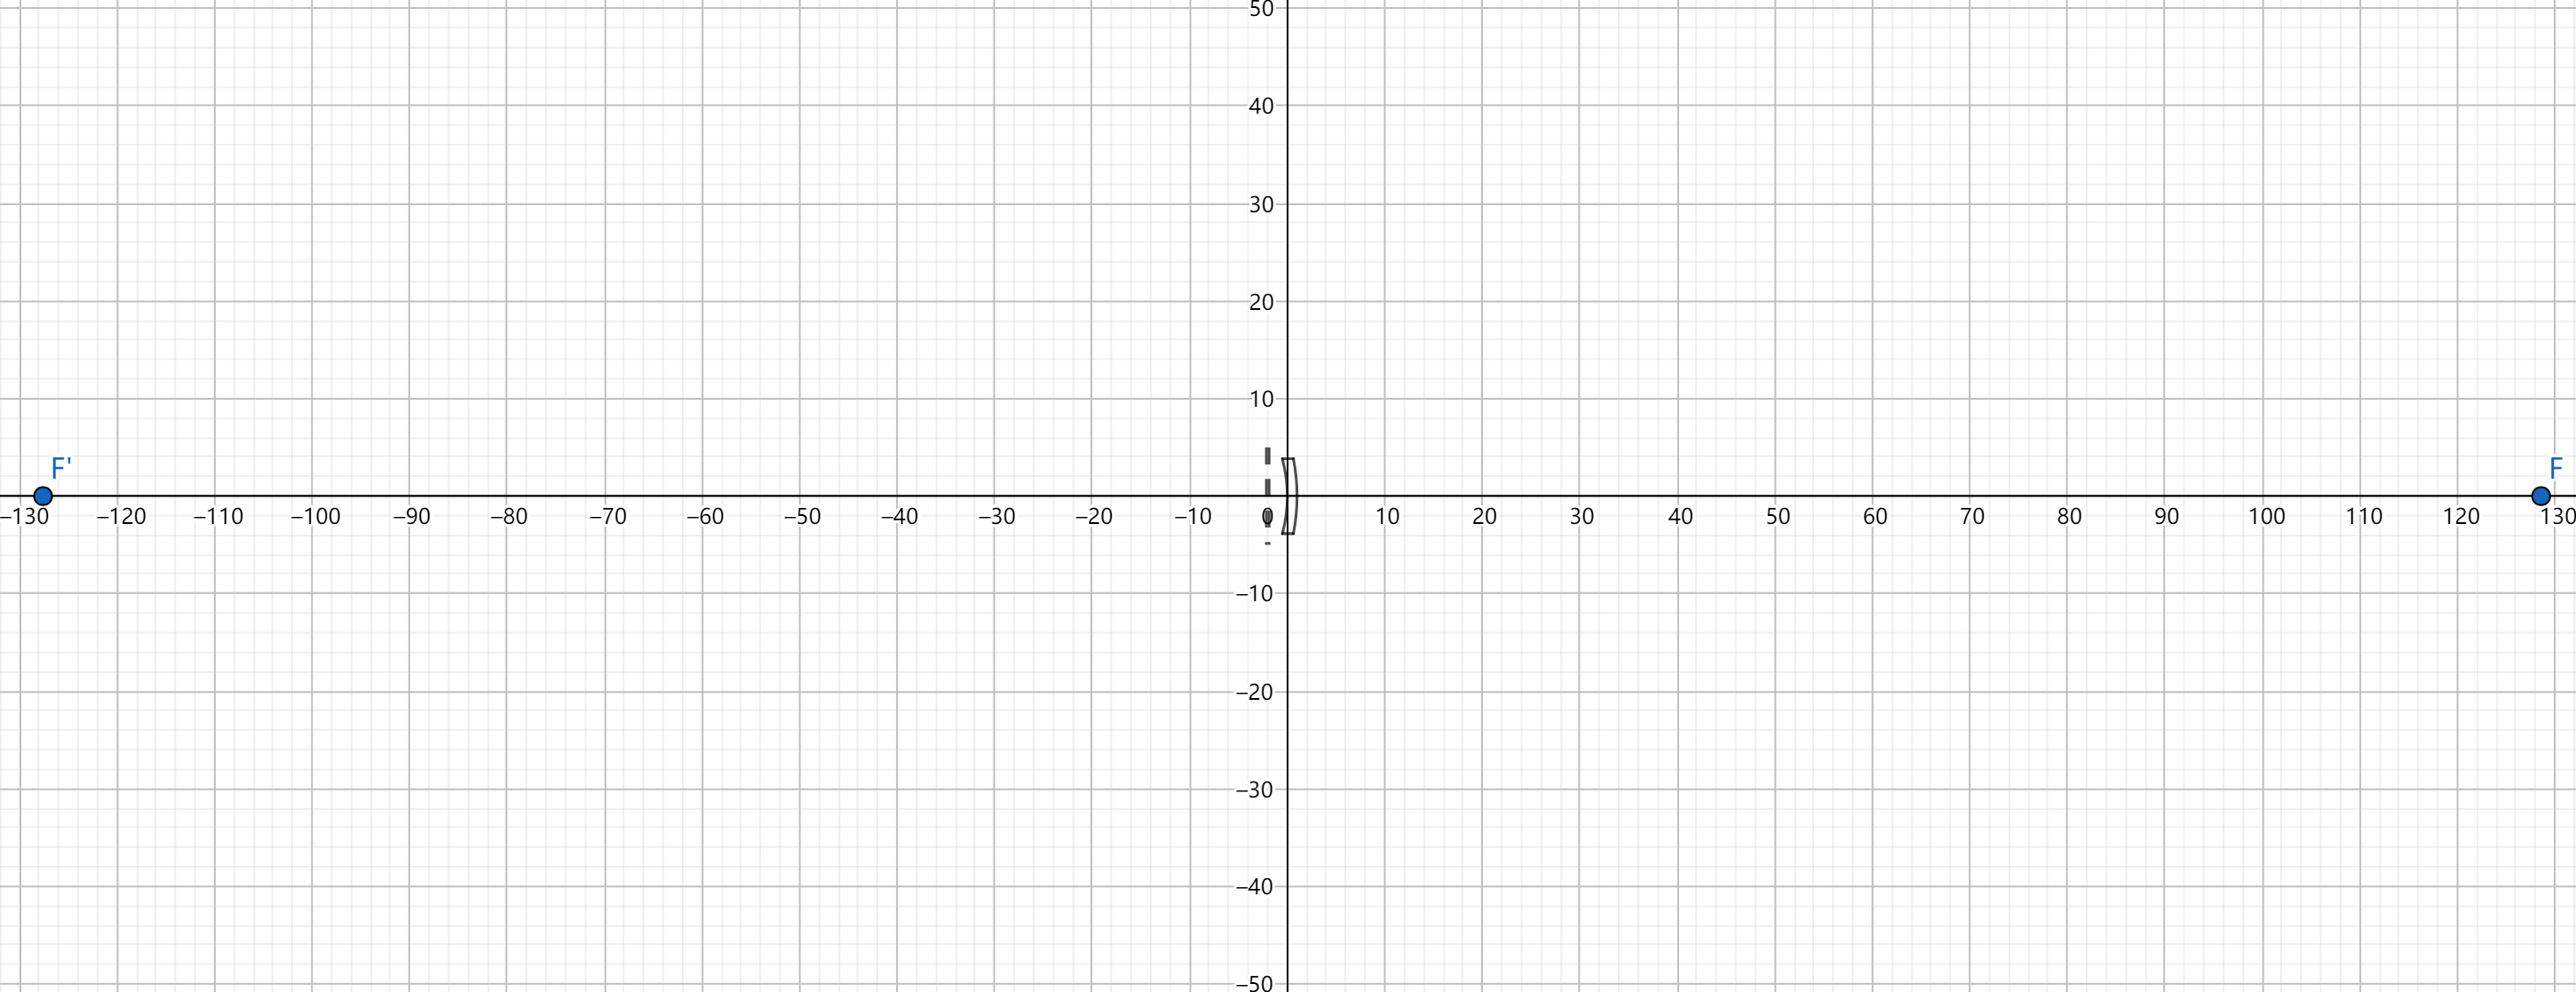
\includegraphics[scale=.2]{OpticsHomework_3Problem_2-32_3(tailored&marked).png}
\caption{题2-32图(3)物方和像方焦点$F,F'$}\label{OpticsHomework_3Problem2-32_3(tailored&marked)}
\end{figure}
\begin{figure}[h]
\centering
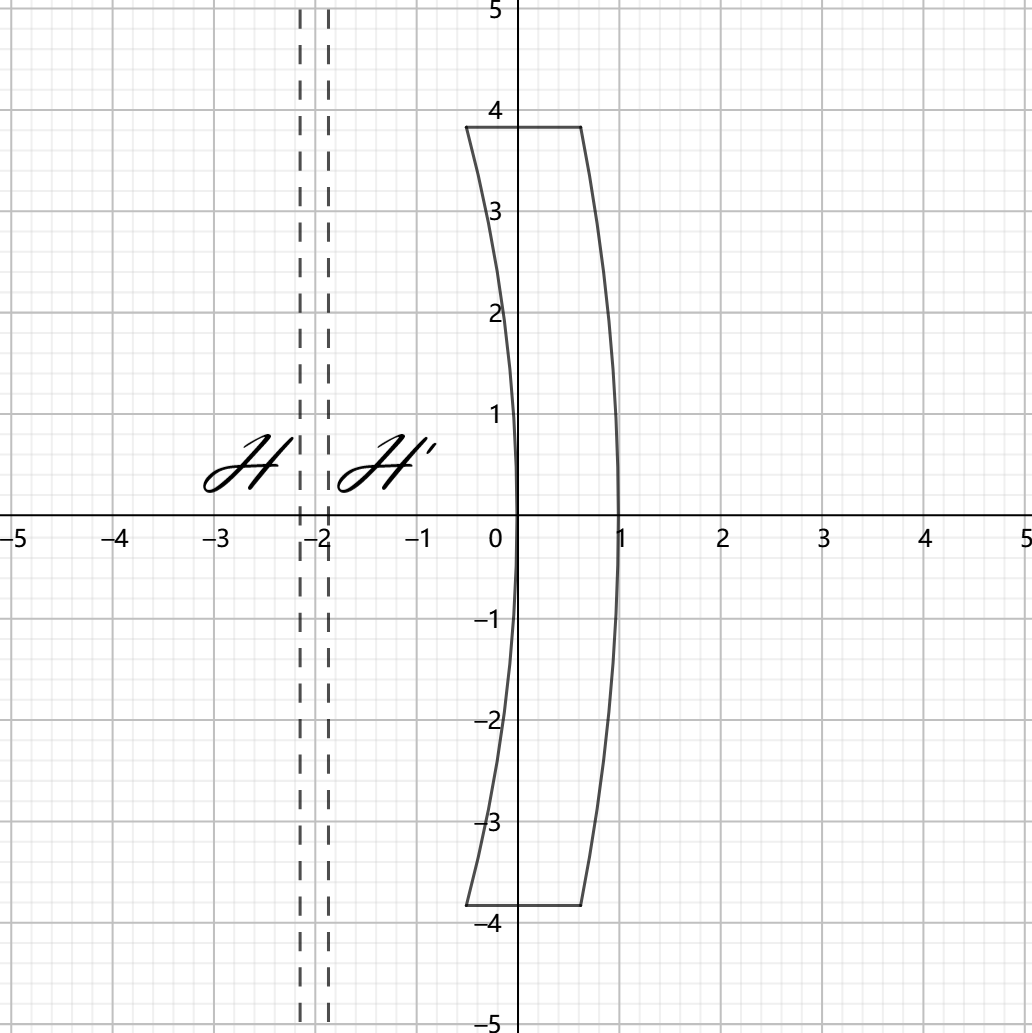
\includegraphics[scale=.3]{OpticsHomework_3Problem_2-32_3(enlarged&tailored&marked).png}
\caption{题2-32图(3)物方和像方主面$\mathscr{H},\mathscr{H}'$}\label{OpticsHomework_3Problem2-32_3(enlarged&tailored&marked)}
\end{figure}
\section*{2-37}证明:
根据牛顿形式的横向放大率公式
\begin{align*}
&V_1 = -\frac{f}{x} = -\frac{x'}{f'}\\
&V_2 = -\frac{f}{x + \Delta x} = -\frac{x' + \Delta x'}{f'}
\end{align*}
以上两式联立消去$x,x'$得到
\begin{align*}
&f = \frac{\Delta x}{\frac{1}{V_1} - \frac{1}{V_2}}\\
&f' = \frac{\Delta x'}{V_1 - V_2}
\end{align*}
\section*{2-40}
\subsection*{(1)}解:
设人眼所能达到的最大物方和像方焦距为$f_{max},f_{max}'$,视网膜到人眼主面之间的距离为$s'$,所配眼镜的焦距为$f_1$(发散透镜,$f_1 < 0$)。未经眼镜矫正前,人眼的物像距公式为
\[
\frac{f_{max}'}{s'} + \frac{f_{max}}{s} = 1
\]
其中$s = 2.5m$。经过眼镜矫正后,人眼和眼镜组成的光具组看无穷远处时达到的像方焦距即为视网膜到人眼主面之间的距离为$s'$,根据理想光具组的联合公式
\[
f' = -\frac{f_1f_{max}'}{\Delta} = s'
\]
其中由于眼镜十分接近人眼,故可近似认为$\Delta = -(f_1 + f_{max})$,以上两式联立解得眼镜的焦距为
\[
f_1 = -s = -2.5m
\]
从而屈光度为
\[
P_1 = \frac{1}{f_1} = -0.4D
\]
故需配$-40$度的眼镜。
\subsection*{(2)}解:
经过眼镜矫正后,明视距离(距人眼$25cm$)处的物体被眼镜成像于$1m$ 处,从而能够被人眼看清,物像距公式为
\[
\frac{1}{-1m} + \frac{1}{0.25m} = \frac{1}{f_2}
\]
解得眼镜的焦距为
\[
f_2 = \frac{1}{3}m
\]
从而屈光度为
\[
P_1 = \frac{1}{f_1} = 3D
\]
故需配$300$度的眼镜。
\section*{2-42}解:
物镜的横向放大率为
\[
V_O = -\frac{x'}{f'} = \frac{160mm}{4mm} = -40
\]
显微镜的总放大率为
\[
M = V_OM_E = -800
\]
\section*{2-45}解:
\subsection*{(1)}对于开普勒型望远镜,其物镜、目镜均为汇聚透镜,$M = -3$,目镜的焦距为
\[
f_E = -\frac{f_O}{M} = 16.7cm
\]
光焦度为
\[
P_E = \frac{1}{f_E} = 6
\]
望远镜为一无焦系统,物镜的像方焦点和目镜的物方焦点重合,物镜、目镜的距离为
\[
\Delta = f_O + f_E = 66.7cm
\]
\subsection*{(2)}对于伽利略型望远镜,其物镜为汇聚透镜,目镜为发散透镜,$M = 3$,目镜的焦距为
\[
f_E = -\frac{f_O}{M} = -16.7cm
\]
光焦度为
\[
P_E = \frac{1}{f_E} = -6
\]
望远镜为一无焦系统,物镜的像方焦点和目镜的物方焦点重合,物镜、目镜的距离为
\[
\Delta = f_O + f_E = 33.3cm
\]
\section*{2-47}解:
出射光瞳即为孔径光阑关于目镜的共轭,目镜的物像距公式为
\[
\frac{1}{s'} + \frac{1}{f_O + f_E} = \frac{1}{f_E}
\]
其中$f_O,f_E$分别为物镜、目镜的焦距,解得出射光瞳与目镜之间的距离为
\[
s' = \frac{f_E(f_O + f_E)}{f_O}
\]
(假设光线从左入射,若$s' > 0$,则出射光瞳在目镜右侧,反之在左侧)

\noindent 出射光瞳直径$D'$与物镜直径$D_0$之比即为孔径光阑关于目镜的横向放大率的绝对值
\[
\frac{D'}{D_0} = |V| = |-\frac{ns'}{n(f_O + f_E)}| = |\frac{f_E}{f_O}| = \frac{1}{|M|}
\]
即
\[
D' = \frac{D_0}{|M|}
\]
\section*{2-49}
\subsection*{(1)}解:
出射光瞳即为孔径光阑关于目镜的共轭,目镜的物像距公式为
\[
\frac{1}{f_O + \Delta + f_E} + \frac{1}{s'} = \frac{1}{f_E}
\]
其中$f_O,f_E$分别为物镜、目镜的焦距,$\Delta$为物镜的像方焦点和目镜的物方焦点之间的距离,解得出射光瞳与目镜之间的距离为
\[
s' = \frac{f_E(f_O + \Delta + f_E)}{f_O + \Delta}
\]
(假设光线从左入射,若$s' > 0$,则出射光瞳在目镜右侧,反之在左侧)
\subsection*{(2)}证明:
\noindent 出射光瞳直径$D'$与物镜直径$D_0$之比即为孔径光阑关于目镜的横向放大率的绝对值
\[
\frac{D'}{D_0} = |V| = |-\frac{ns'}{n(f_O + \Delta + f_E)}| = |\frac{f_E}{f_O + \Delta}|
\]
成像时物在物镜的物方焦点附近,故在傍轴近似下
\[
D_0 \approx 2f_O'u_0
\]
其中$u_0$是入射孔径角,而$f_O'$代表物镜的物方焦距,这是因为在油浸物镜等情况下,物镜在物方的焦距有别于其在真空中的焦距
\[
f_O' = nf_O
\]
其中$n$是物方的折射率。
以上各式联立得到
\[
D' = \frac{2nf_Of_Eu_0}{f_O + \Delta}
\]
显微镜的视角放大率为
\[
M = -\frac{s_0\Delta}{f_Of_E}
\]
又由于物镜焦距远小于镜筒长,故有近似$f_O + \Delta \approx \Delta$,从而傍轴近似下出射光瞳的直径与入射孔径角$u_0$之间的关系为
\[
D' = \frac{2s_0u_0}{|M|}
\]
\section*{2-50}解:
$DD$关于$L_1$的物像距公式
\begin{align*}
&\frac{1}{l} + \frac{1}{s'} = \frac{1}{f_1}\\
&\Longrightarrow s' = 4a
\end{align*}
$DD$关于$L_1$的共轭的半径为
\[
r' = |\frac{1}{V'}|r_3 = |\frac{s}{l}|r_3 = r_3
\]
由于$\frac{r'}{s - s'} = \frac{r_3}{6a} < \frac{r_1}{s} = \frac{3r_3}{10a}$,故$DD$关于$L_1$的共轭即为此光具组的入射光瞳,故此光具组的入射光瞳位于$L_1$ 左侧$4a$处,半径为$r_3$。

\noindent $DD$关于$L_2$的物像距公式
\begin{align*}
&\frac{1}{s''} + \frac{1}{d - l} = \frac{1}{f_3}\\
&\Longrightarrow s'' = 2a
\end{align*}
$DD$关于$L_2$的共轭的半径为
\[
r'' = |V''|r_3 = \frac{s''}{d - l}r_3 = r_3
\]
光具组的焦距为
\[
f = \frac{f_1f_2}{d - f_1 - f_2} = \frac{2}{3}a
\]
物点$Q$关于光具组的共轭的位置为
\begin{align*}
&\frac{1}{s_1} + \frac{1}{s} = \frac{1}{f_1}\\
&s_1 + s_2 = d\\
&\frac{1}{s_3} + \frac{1}{s_2} = \frac{1}{f_2}\\
&\Longrightarrow s_3 = \frac{5}{7}a
\end{align*}
由于$\frac{r''}{s'' - s_3} = \frac{5r_3}{3a} < \frac{r_2}{s_3} = \frac{15r_3}{7a}$,故$DD$关于$L_2$的共轭即为此光具组的出射光瞳,故此光具组的入射光瞳位于$L_2$右侧$2a$处,半径为$r_3$。

\noindent 光阑$DD$为此光具组的孔径光阑,故此光具组的孔径光阑位于$L_1$右侧$4a$处,半径为$r_3$。

\noindent $L_1,L_2$对于$DD$中心的张角分别为
\begin{align*}
&u_1 = \arctan\frac{r_1}{l} = \frac{3r_3}{4a}\\
&u_2 = \arctan\frac{r_2}{d - l} = \frac{3r_3}{2a}
\end{align*}
由于$u_1 < u_2$,故$L_4$既是此光具组的入射窗,又是视场光阑,其半径为$r_1 = 3r_3$。
\section*{2-54}解:
对于$F$线和$C$线,根据磨镜者公式和密接复合透镜组光焦度为各透镜光焦度之和的规律,胶合透镜的光焦度分别为
\begin{align*}
&P_F = P_{1F} + P_{2F} = (n_{1F} - 1)K_1 + (n_{2F} - 1)K_2\\
&P_C = P_{1C} + P_{2C} = (n_{1C} - 1)K_1 + (n_{2C} - 1)K_2
\end{align*}
其中$K_1 = \frac{1}{r_1} - \frac{1}{r_2}, K_2 = \frac{1}{r_2} - \frac{1}{r_3}$,$r_1$代表冕牌玻璃$K9$的非黏合面的曲率半径,$r_2$代表两种介质粘合面的曲率半径,$r_3$代表重火石玻璃$F4$的非黏合面的曲率半径。
要消除$F$线和$C$线的焦距色差,则
\[
P_F - P_C = (n_{1F} - n_{1C})K_1 + (n_{2F} - n_{2C})K_2 = 0
\]
同时,对于$D$线,焦距为$100mm$,即
\[
P_D = P_{1D} + P_{2D} = (n_{1D} - 1)K_1 + (n_{2D} - 1)K_2 = 10(D)
\]
以上各式联立解得
\begin{align*}
&K_1 = \frac{1}{r_1} - \frac{1}{r_2} = \frac{10(n_{2F} - n_{2C})}{(n_{2F} - n_{2C})(n_{1D} - 1) - (n_{1F} - n_{1C})(n_{2D} - 1)} = 44.911D\\
&K_2 = \frac{1}{r_2} - \frac{1}{r_3} = \frac{10(n_{1F} - n_{1C})}{(n_{1F} - n_{1C})(n_{2D} - 1) - (n_{2F} - n_{2C})(n_{1D} - 1)} = -21.274D
\end{align*}
假设以冕牌玻璃$K9$做负透镜而重火石玻璃$F4$做正透镜,则$r_1 \to \infty$,解得
\begin{align*}
&r_2 = -2.2266cm\\
&r_3 = -4.2306cm
\end{align*}
$r_2 < 0$与假设不符,舍去。

\noindent 假设以冕牌玻璃$K9$做正透镜而重火石玻璃$F4$做负透镜,则$r_1 \to \infty$,解得
\begin{align*}
&r_2 = 4.2306cm\\
&r_3 = -4.7007cm
\end{align*}
\end{document}
